%\subsection{Effect of lens radius}
%lensed_waveguide_radium
In this part the effect of the radius of the lens interface for the waveguide will be discussed. We are going to keep the height of the lens on the waveguide and change the lens radius. In Tab. \ref{tab:coupling_lensed_waveguide_radium} the lens height is chosen for $1\mu$m, $1.5\mu$m and $2\mu$m respectively. We expand the lens radius from $2\mu$m to $3.6\mu$m and observe $|S21|$ as coupling efficiency.\\

\begin{table}
\caption{Cupling efficiency between TLF and lensed waveguide due to changing the lens radius}
\centering
\begin{tabular}{|c|c|c|c|}
\hline
\multirow{2}*{Radius($\mu$m)}&\multicolumn{3}{c|}{Height($\mu$m)}\\
\cline{2-4}
 								&	1&	1.5&2\\
\hline
$2.0$& $59.5\%$	&$61.3\%$	&$69\%$\\
$2.2$& $59\%$		&$60.8\%$	&$68.3\%$\\
$2.4$&$59\%$		&$60.3\%$	&$66.8\%$\\
$2.6$&$58.6\%$	&$59.9\%$	&$65.3\%$\\
$2.8$&$58.2\%$	&$59.3\%$	&$64\%$\\
$3.0$&$57.8\%$	&$58.7\%$	&$63\%$\\
\hline
\end{tabular}
\label{tab:coupling_lensed_waveguide_radium}
\end{table}

According the data in Tab. \ref{tab:coupling_lensed_waveguide_radium} the coupling behavior curve can be mapped in Fig. \ref{fig:coupling_lenses_curve_rxx}. Apparently, it can be told that the coupling efficiencies under different lens heights are monotonously declining due to the variation of the lens radius.
\begin{figure}[!ht]
\centering
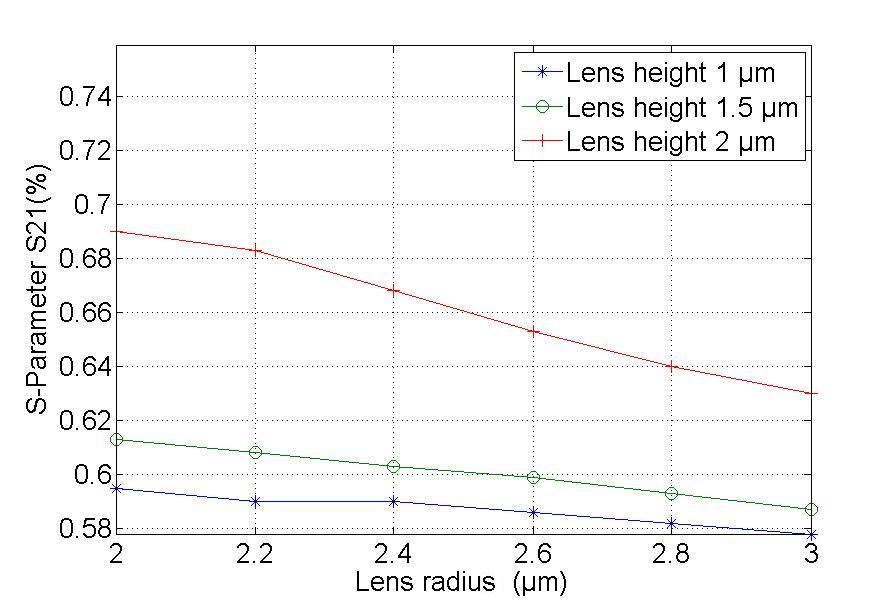
\includegraphics[width=0.8\textwidth]{bilder/s21_fix_lens_height_rxx}
\caption{Coupling efficiency due to changing the lens radius}
\label{fig:coupling_lenses_curve_rxx}
\end{figure}
\begin{figure}[!ht]
\centering
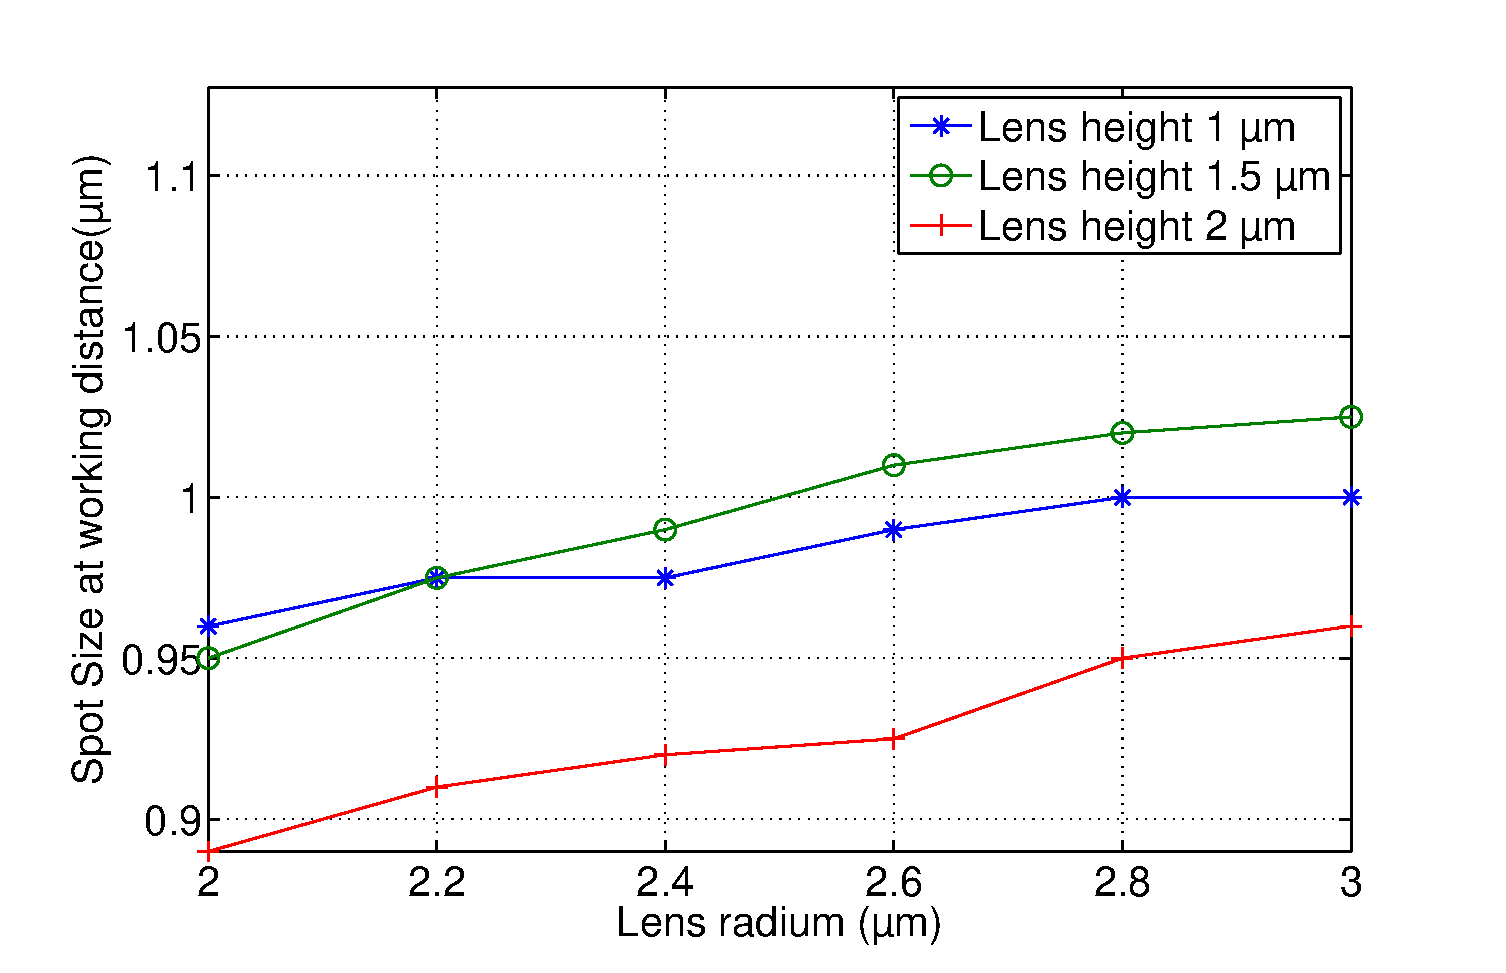
\includegraphics[width=0.8\textwidth]{bilder/spot_fix_lens_height_rxx}
\caption{The spot size curve at lensed waveguide interface due to changing lens height}
\label{fig:lensed_guide_spot_size_curve_rxx}
\end{figure}
Meanwhile the spot size curve in Fig. \ref{fig:lensed_guide_spot_size_curve_rxx} along the variation of the lens radius behave inversely in compare with the trends of coupling efficiency. These simulation results bring us the conclusion that the smallest lens radius gains the best coupling efficiency when the lens height is fixed. 
